% D_Report_sec6-7_20261102.tex —— 第 6 章 + 7.1 节（D 负责部分）
% 所有数字均与 results/*.csv 核对过；图在同级目录 fig_6_1..fig_6_4。
% 编译: pdfLaTeX / XeLaTeX 均可（Overleaf 直接编译）; Word 版由 pandoc 转出。
\documentclass[12pt]{article}
\usepackage[a4paper,margin=1in]{geometry}
\usepackage{booktabs}
\usepackage{graphicx}
\usepackage{amsmath}
\setlength{\tabcolsep}{4pt}
\setlength{\emergencystretch}{2em}
\begin{document}

\section*{6 Results and Evaluation}

The main matrix compares four classifiers under plain, SMOTE, cost-sensitive and
threshold-adjusted training. Metrics refer to \texttt{bad} on credit-g and
\texttt{sick} on sick. Section 6.1 reports model selection and metric choice;
Section 6.2 tests strategy effects; Section 6.3 examines preprocessing;
Section 6.4 evaluates holdout errors; Section 6.5 adds exploratory evidence.
Data preparation and validation are defined in Sections 3 and 5.

\subsection*{6.1 Main Results across Two Datasets}

\begin{center}
\begin{minipage}{\textwidth}
\centering
{\footnotesize\textbf{Table 6.1}\ \ credit-g positive-class F1 under ten-fold CV}

\footnotesize
\begin{tabular}{p{1.35in}p{0.95in}p{0.95in}p{0.95in}p{0.95in}}
\toprule
Model & Plain & SMOTE & Cost-sensitive & Threshold \\
\midrule
Decision Tree & $0.322 \pm 0.192$ & $0.471 \pm 0.078$ & $0.523 \pm 0.030$ & $0.561 \pm 0.038$ \\
Random Forest & $0.499 \pm 0.079$ & $0.509 \pm 0.077$ & $0.595 \pm 0.064$ & $0.595 \pm 0.059$ \\
Logistic Regression & $0.531 \pm 0.060$ & $0.591 \pm 0.051$ & $\mathbf{0.597 \pm 0.034}$ & $0.591 \pm 0.049$ \\
SVC & $0.498 \pm 0.101$ & $0.560 \pm 0.050$ & $0.593 \pm 0.032$ & $0.590 \pm 0.055$ \\
\midrule
\multicolumn{5}{l}{ZeroR reference: F1 $=0$; accuracy $=0.700$; recall $=0$} \\
\bottomrule
\end{tabular}
\end{minipage}
\end{center}

\begin{center}
\begin{minipage}{\textwidth}
\centering
{\footnotesize\textbf{Table 6.2}\ \ sick positive-class F1 under ten-fold CV}

\footnotesize
\begin{tabular}{p{1.35in}p{0.95in}p{0.95in}p{0.95in}p{0.95in}}
\toprule
Model & Plain & SMOTE & Cost-sensitive & Threshold \\
\midrule
Decision Tree & $0.836 \pm 0.050$ & $0.747 \pm 0.050$ & $0.836 \pm 0.050$ & $0.820 \pm 0.048$ \\
Random Forest & $0.870 \pm 0.047$ & $\mathbf{0.897 \pm 0.051}$ & $0.873 \pm 0.048$ & $0.877 \pm 0.052$ \\
Logistic Regression & $0.687 \pm 0.091$ & $0.521 \pm 0.028$ & $0.687 \pm 0.091$ & $0.745 \pm 0.038$ \\
SVC & $0.763 \pm 0.064$ & $0.742 \pm 0.039$ & $0.763 \pm 0.064$ & $0.809 \pm 0.039$ \\
\midrule
\multicolumn{5}{l}{ZeroR reference: F1 $=0$; accuracy $=0.939$; recall $=0$} \\
\bottomrule
\end{tabular}
\end{minipage}
\end{center}

Values are means $\pm$ population SD across ten folds; bold marks the
highest mean in each main matrix. Credit-g uses 5:1 cost weights; sick uses an
equal-cost 1:1 control. Source: \texttt{results/all\_metrics\_v1.csv}.

\begin{enumerate}
\item \textbf{The best combination changes with the dataset.} Cost-weighted Logistic
Regression leads credit-g; Random Forest with SMOTE leads sick. Figure 6.1 visualises
the complete matrices, including the variability across model--strategy combinations.
\item \textbf{Minority detection requires more than accuracy.} ZeroR predicts the
majority label throughout. Its high accuracy and zero recall justify evaluating
positive-class F1, precision and recall alongside the task-specific cost.
\item \textbf{The same intervention can help or harm.} Every intervention raises
credit-g F1 relative to its own plain model. On sick, SMOTE lowers F1 for DT, LR and
SVC. For LR, recall rises from 0.606 to 0.870 but precision falls from 0.803 to 0.373:
detecting more positives does not guarantee a better F1.
\item \textbf{Ranking curves and classification errors are complementary.} The RF
curves in Figure 6.2 are similar across plain, SMOTE and equal-cost training. This is
an observation for these configurations. Threshold adjustment preserves the same
fitted scores by construction. Pooled curve statistics and fold-averaged table
metrics use different aggregation.
\end{enumerate}

\begin{center}
\begin{minipage}{\textwidth}
\centering
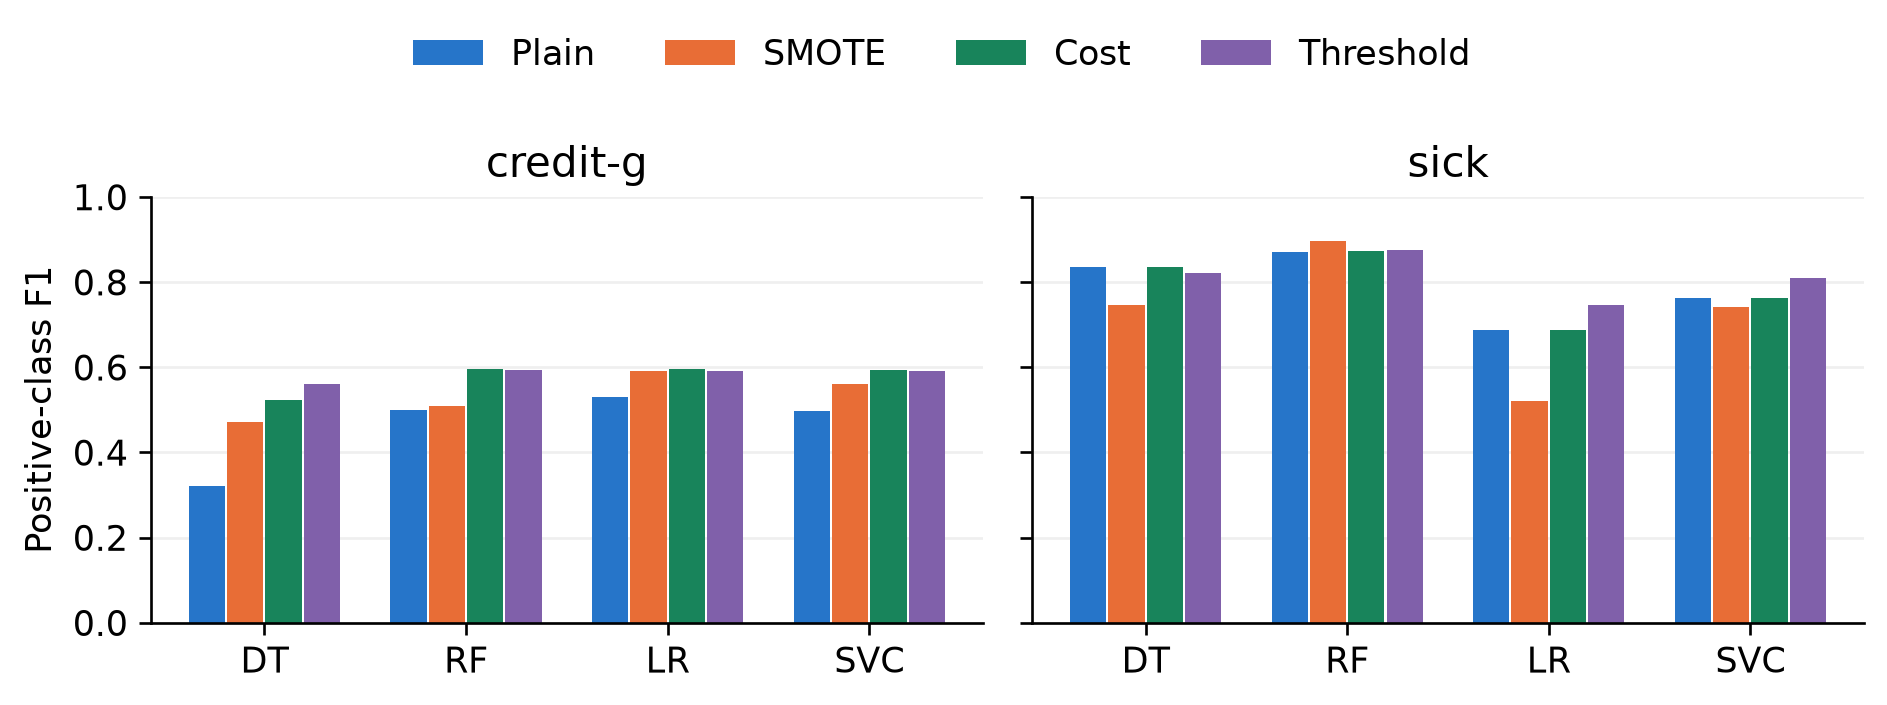
\includegraphics[width=\textwidth]{fig_6_1_main_f1.png}

{\footnotesize\textbf{Figure 6.1}\ \ Mean F1 for the complete main matrices. DT = Decision
Tree; RF = Random Forest; LR = Logistic Regression. All scores use ten-fold CV. SDs
are retained in Tables 6.1--6.2. Source: \texttt{all\_metrics\_v1.csv}.}
\end{minipage}
\end{center}

\begin{center}
\begin{minipage}{\textwidth}
\centering
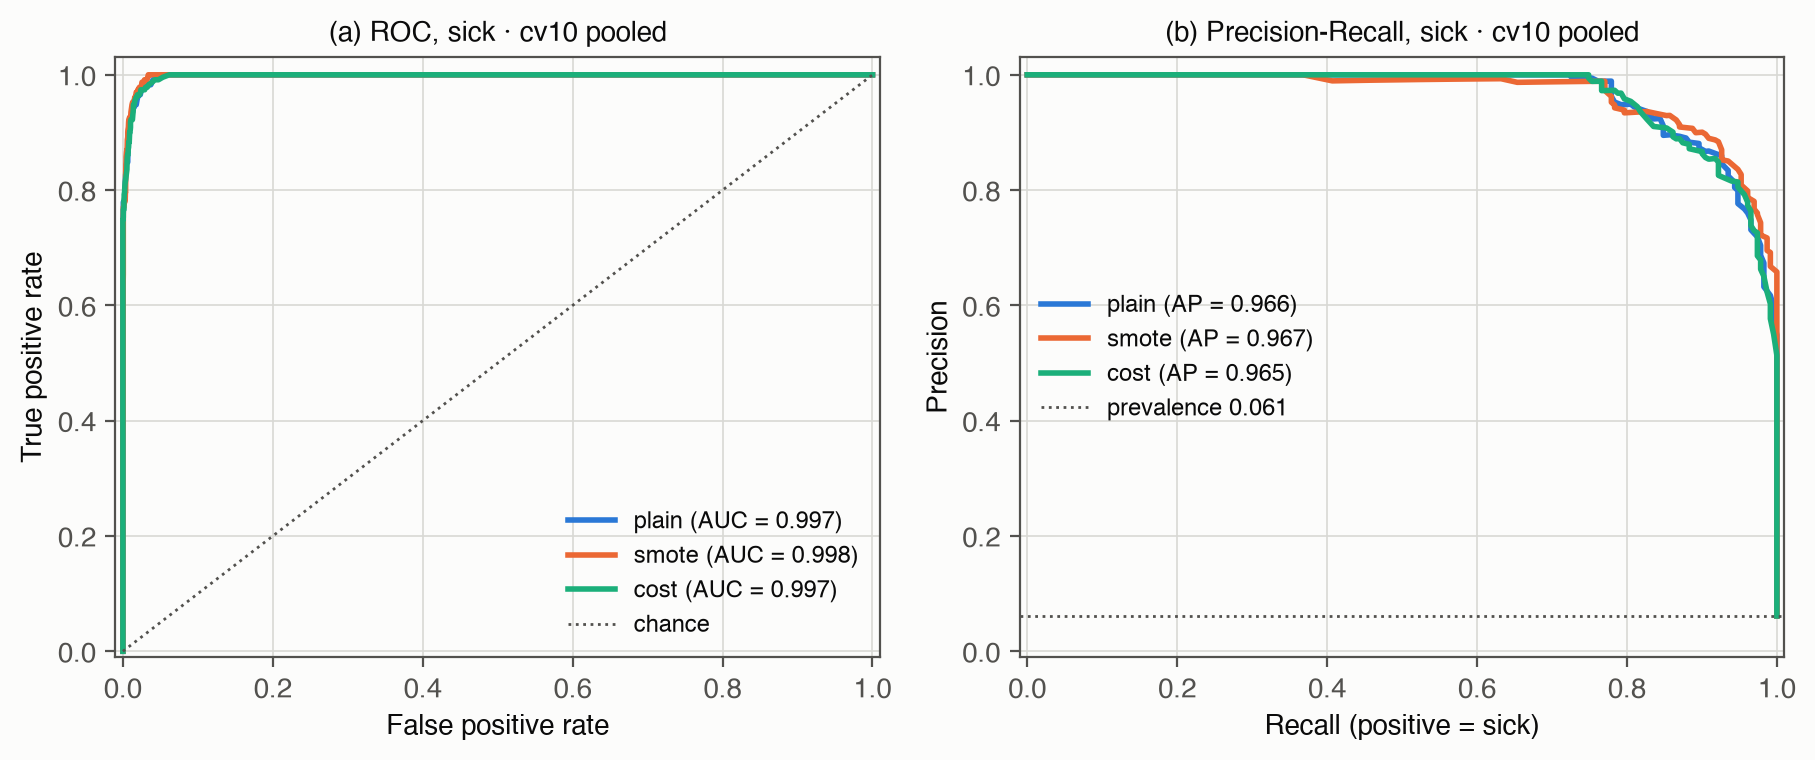
\includegraphics[width=0.88\textwidth]{fig_6_2_roc_pr.png}

{\footnotesize\textbf{Figure 6.2}\ \ RF ROC and precision--recall curves on sick. All 3,772
out-of-fold predictions are pooled; positive = sick. AP denotes average precision.
Dotted lines mark chance and prevalence. Source:
\texttt{results/preds/sick\_rf\_*\_cv10\_preds.csv}.}
\end{minipage}
\end{center}

\subsection*{6.2 Strategy Effects and Statistical Evidence}

\begin{center}
\begin{minipage}{\textwidth}
\centering
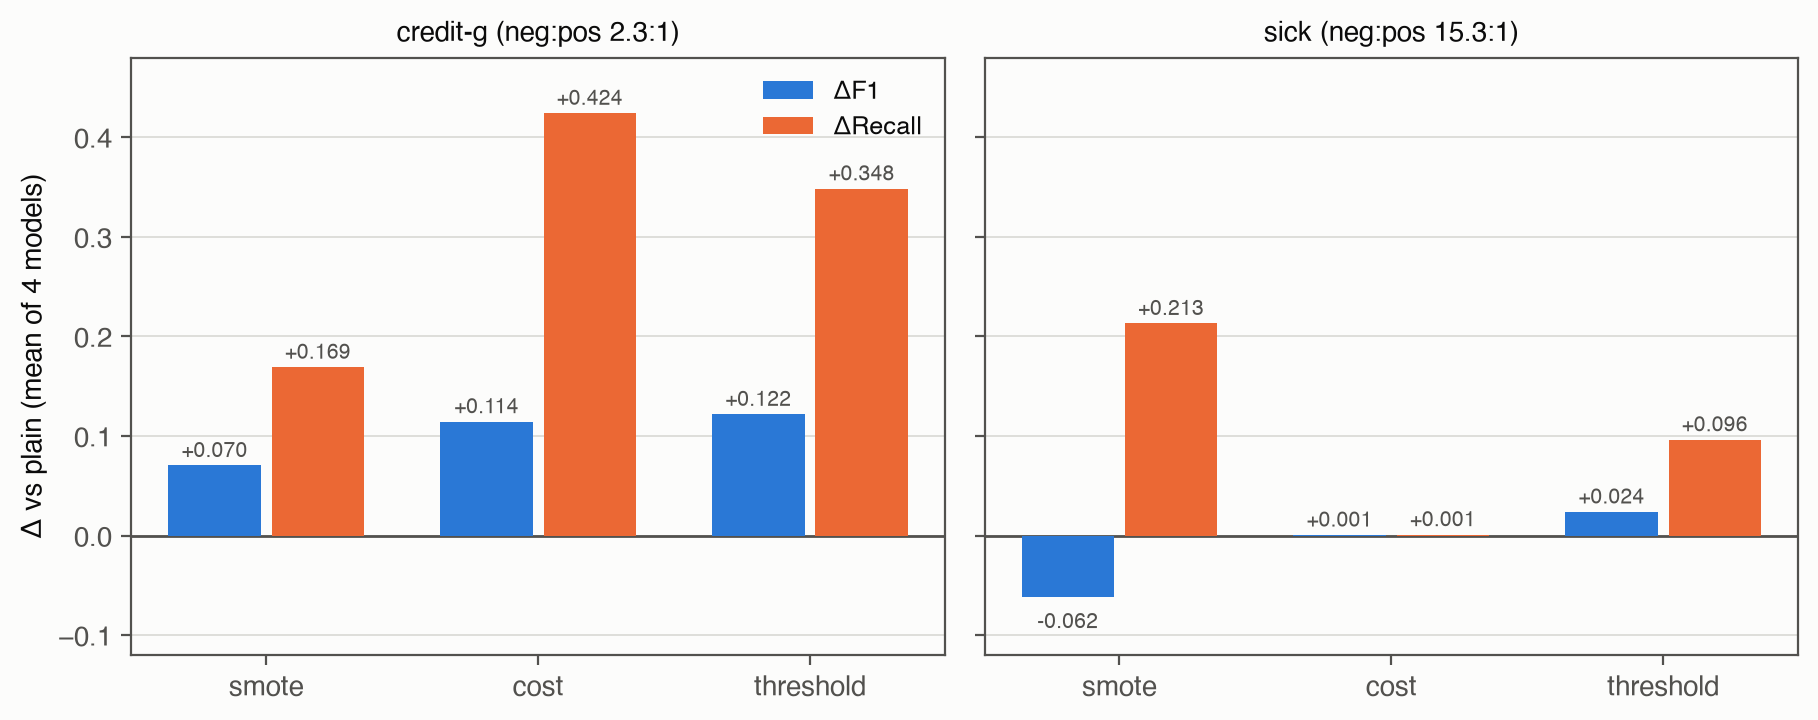
\includegraphics[width=\textwidth]{fig_6_3_strategy_gain.png}

{\footnotesize\textbf{Figure 6.3}\ \ Mean change from plain training across four classifiers,
using ten-fold CV. These are descriptive changes, not significance tests. Ratios
denote negative:positive counts. Source: \texttt{cross\_dataset\_comparison\_v1.csv}.}
\end{minipage}
\end{center}

\begin{center}
\begin{minipage}{\textwidth}
\centering
{\footnotesize\textbf{Table 6.3}\ \ Counts of significant strategy-versus-plain contrasts}

\footnotesize
\begin{tabular}{p{0.8in}p{0.75in}p{0.75in}p{0.95in}p{0.9in}}
\toprule
Dataset & Metric & Tested & Raw $p<.05$ & Holm $p<.05$ \\
\midrule
credit-g & F1 & 12 & 3 & 0 \\
sick & F1 & 12 & 2 & 0 \\
credit-g & Recall & 12 & 11 & 8 \\
sick & Recall & 12 & 7 & 2 \\
\bottomrule
\end{tabular}
\end{minipage}
\end{center}

Following the corrected paired-test procedure of Section 5, Nadeau--Bengio corrected
paired $t$-tests account for the overlap of training folds, and the Holm adjustment is
applied over all 120 pairwise contrasts among the 16 configurations, separately for
each dataset and metric; Table 6.3 reports the twelve pre-specified within-model
strategy contrasts from each family. Source: \texttt{results/ttest/}.

\begin{enumerate}
\item \textbf{Recall has stronger statistical support.} Across both datasets, recall
increases in 21 contrasts and is unchanged in three. Ten of 24 recall contrasts
survive Holm correction; none of the 24 F1 contrasts does. The highest observed F1 is
therefore a selection criterion, not proof of significant superiority.
\item \textbf{Averaging hides important exceptions.} Figure 6.3 summarises the overall
pattern. Table 6.2 identifies four sick F1 losses: SMOTE with DT, LR and SVC, and
threshold adjustment with DT. Model-specific results remain necessary when selecting
a strategy.
\item \textbf{Non-significance is not equivalence.} The conservative correction limits
claims about improvements; it does not establish that configurations perform equally.
Recall, precision and the error-cost objective should be considered together.
\end{enumerate}

\subsection*{6.3 Cross-Dataset Comparison and Preprocessing Evidence}

\begin{center}
\begin{minipage}{\textwidth}
\centering
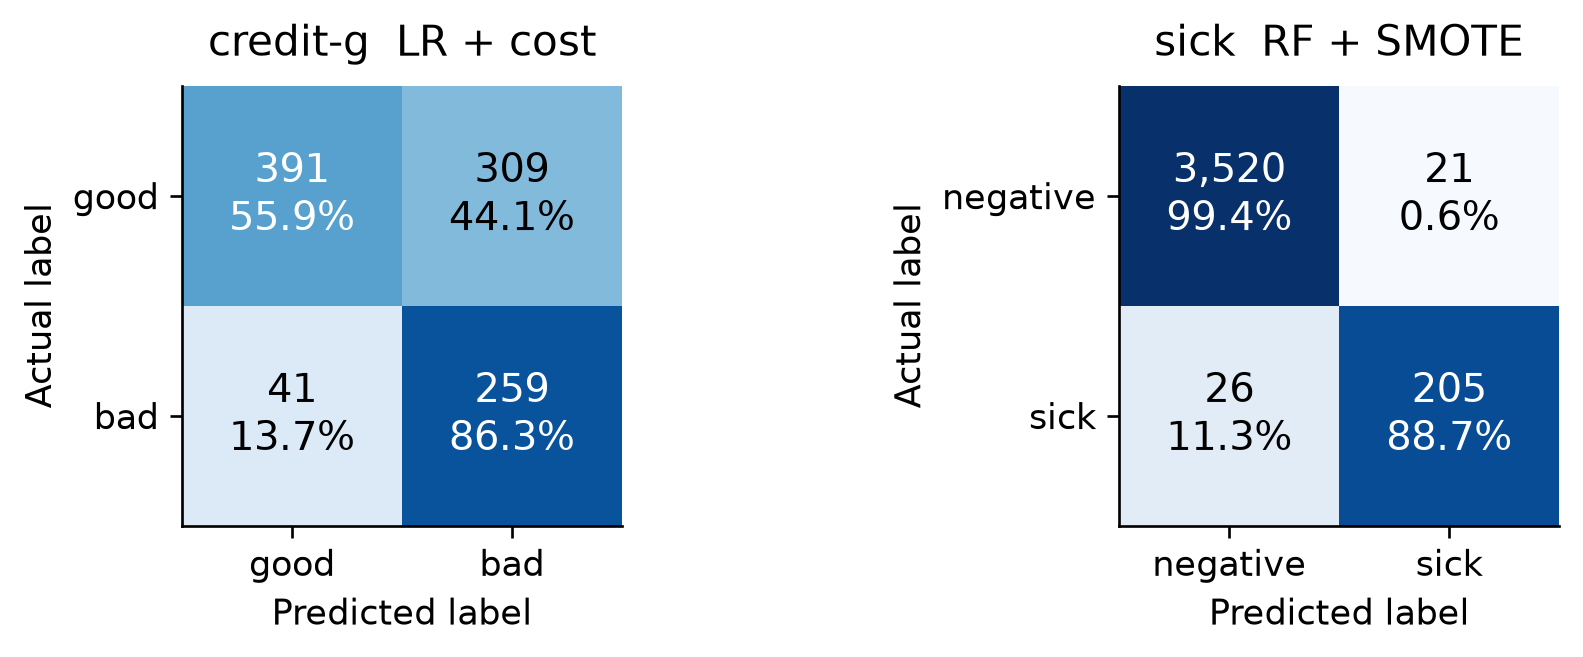
\includegraphics[width=\textwidth]{fig_6_4_confusion.png}

{\footnotesize\textbf{Figure 6.4}\ \ Main-matrix winners, pooled ten-fold CV. Each cell gives
count and percentage within its actual class. Rows = actual; columns = predicted.
Positive labels: \texttt{bad} and \texttt{sick}. Source: \texttt{all\_metrics\_v1.csv}.}
\end{minipage}
\end{center}

\begin{enumerate}
\item \textbf{The selected models carry different error burdens.} In Figure 6.4 the
credit-g champion identifies 86.3\% of bad records but flags 44.1\% of good ones;
the sick champion identifies 88.7\% of positives with only 0.6\% false alarms among
negatives (counts in Figure 6.4). Both winners were selected by F1, yet their error
profiles differ sharply; Section 6.4 evaluates the decision trade-offs of both
configurations. The simultaneous differences in size, attributes, missingness and
imbalance (Section 3) prevent isolating a single cause.
\item \textbf{Encoding evidence supports a specific LR choice.} Credit-g LR gives F1
0.531 with one-hot, 0.406 with ordinal and 0.415 with standardised ordinal encoding.
This supports the tested LR pipeline. Categorical interpolation is a hypothesis for
SMOTE losses.
\item \textbf{Missing-data handling trades retention against performance.} For
Decision Tree on sick under stratified ten-fold CV: fold-internal imputation scores
F1 $0.830 \pm 0.049$ with AUC $0.974$; dropping the 1,129 incomplete records ---
19 of the 231 positives among them --- scores $0.843 \pm 0.069$ with AUC $0.964$;
treating ``missing'' as its own category scores F1 0.828 with AUC 0.965. Deletion
nominally leads on F1 but sits within one standard deviation of imputation while
discarding those records; imputation preserves every positive and posts the best AUC.
Decision: impute inside the pipeline. Overlapping spreads and changed samples
preclude a stricter equivalence claim. Source:
\texttt{results/b4\_missing\_comparison.csv}.
\end{enumerate}

\subsection*{6.4 Holdout Results and Decision Trade-offs}

\begin{center}
\begin{minipage}{\textwidth}
\centering
{\footnotesize\textbf{Table 6.4}\ \ Main-matrix winners on the fixed 70:30 holdout}

\footnotesize
\begin{tabular}{p{0.75in}p{1.15in}p{0.9in}p{0.65in}p{0.8in}p{0.55in}p{0.55in}}
\toprule
Dataset & Configuration & N / positive & Recall & Precision & F1 & Cost \\
\midrule
credit-g & LR + cost & 300 / 90 & 0.822 & 0.448 & 0.580 & 0.570 \\
sick & RF + SMOTE & 1,132 / 69 & 0.957 & 0.868 & 0.910 & --- \\
\bottomrule
\end{tabular}
\end{minipage}
\end{center}

Credit-g cost follows Section 5; sick has no official cost matrix.
Source: holdout rows of \texttt{all\_metrics\_v1.csv}.

\begin{enumerate}
\item \textbf{Decisions have measurable trade-offs.} Credit-g LR + cost misses 16
bad-labelled records and flags 91 good-labelled records. Cost falls to 0.570 from
0.887 for plain LR and 1.500 for ZeroR. RF + threshold has lower cost at 0.543, so F1
selection is not cost minimisation. Sick RF + SMOTE produces three misses and ten
false alarms.
\item \textbf{Holdout is an internal assessment.} Full-data CV informed selection; the
overlapping holdout is not an independent final test. These historical benchmarks do
not establish deployment readiness.
\end{enumerate}

\subsection*{6.5 Exploratory Ensembles and Association Rules}

\begin{center}
\begin{minipage}{\textwidth}
\centering
{\footnotesize\textbf{Table 6.5}\ \ Complete exploratory ensemble results under ten-fold CV}

\footnotesize
\begin{tabular}{p{0.75in}p{1.3in}p{1.05in}p{0.65in}p{0.55in}p{0.55in}}
\toprule
Dataset & Configuration & $\text{F1 mean} \pm \text{SD}$ & Recall & AUC & Time s \\
\midrule
credit-g & Bagging + plain & $0.510 \pm 0.072$ & 0.430 & 0.782 & 2.2 \\
credit-g & Bagging + SMOTE & $\mathbf{0.548 \pm 0.074}$ & 0.560 & 0.770 & 1.2 \\
credit-g & AdaBoost + plain & $0.499 \pm 0.070$ & 0.473 & 0.735 & 1.2 \\
credit-g & AdaBoost + SMOTE & $0.501 \pm 0.087$ & 0.483 & 0.723 & 2.4 \\
sick & Bagging + plain & $0.819 \pm 0.050$ & 0.775 & 0.990 & 3.6 \\
sick & Bagging + SMOTE & $0.785 \pm 0.037$ & 0.987 & 0.994 & 4.6 \\
sick & AdaBoost + plain & $0.918 \pm 0.045$ & 0.901 & 0.999 & 9.5 \\
sick & AdaBoost + SMOTE & $\mathbf{0.937 \pm 0.043}$ & 0.931 & 0.999 & 28.9 \\
\bottomrule
\end{tabular}
\end{minipage}
\end{center}

Bold marks each dataset's highest exploratory mean. Time is recorded
fitting time. These configurations are outside the main statistical family. Source:
\texttt{ensemble\_metrics\_v1.csv}.

\begin{enumerate}
\item \textbf{High recall does not guarantee a better balance.} On sick, Bagging +
SMOTE pushes recall to 0.987 while F1 falls to 0.785 (plain 0.819); AdaBoost + SMOTE
instead keeps recall at 0.931 with F1 0.937, the highest exploratory mean, though its
gap to the main-matrix winner RF + SMOTE (0.897) was not tested. Among the four
exploratory tests outside the main Holm family, only sick AdaBoost plain versus DT +
SMOTE meets the raw threshold ($p = 0.000639$). The precision--recall trade-off
depends on the model, even under the same resampling strategy.
\item \textbf{Rules add a different interpretation.} The highest-duration bin with
savings below 100 covers 124 records, including 71 bad labels: confidence 0.573 and
lift 1.91. Six rules meet confidence $\geq 0.50$ and a five-percentage-point gain over
the stronger single-condition rule. Some fields recur in tree interpretations, but no
complete selected rule is reproduced. Apriori uses all 1,000 records; the trees use
700 training records. Their overlap is complementary interpretation, not independent
validation.
\end{enumerate}

\section*{7 Conclusion and Future Work}

\subsection*{7.1 Findings}

\begin{enumerate}
\item \textbf{(RQ1) Selection depends on the dataset.} Cost-weighted LR leads the
credit-g main matrix at F1 0.597; RF + SMOTE leads sick at 0.897. Section 6.2 supports
recall gains more strongly than F1 gains. No intervention improves every model on both
datasets.
\item \textbf{(RQ2) Accuracy needs minority-class evidence.} The reference rows in
Tables 6.1--6.2 illustrate the limitation of accuracy. Positive-class precision, recall
and F1, together with relevant error costs, reveal the decision trade-offs.
\item \textbf{(RQ3) One-hot encoding favours the tested LR pipeline; imputation
preserves sick records.} One-hot reaches F1 0.531 against 0.406 with ordinal codes on
credit-g LR; imputation retains all 3{,}772 sick records with the best AUC among the
three tested missing-data schemes (0.974). These conclusions are scoped to the tested
configurations; dataset differences and shared explanatory fields do not establish
causal mechanisms.
\item \textbf{(RQ4) The champions cut holdout cost and missed positives.} On the
holdout, credit-g cost falls to 0.570 from 0.887 for plain LR and 1.500 for
always-approve ZeroR, and the sick champion misses 3 of 69 positives with ten false
alarms. Section 6.4 bounds these results to internal evaluation because model
selection and final testing were not fully independent.
\end{enumerate}

\end{document}
